\documentclass[journal]{IEEEtran}

\usepackage{cite}
\usepackage{graphicx}
\usepackage{array}

\newcommand{\blurb}[1]{\marginpar{{\tt !!!}}{\tt [... #1 ...]}}

\begin{document}

\title{A Second Screen Architecture for Capturing Viewers' Interaction Data in TV Environments}
\author{Ricardo~Erikson~V.~de~S.~Rosa,\IEEEmembership{Student Member, IEEE,} 
	and Vicente~Ferreira~de~Lucena~Jr.,\IEEEmembership{Senior Member,IEEE}
	% and~Lucas~Carvalho~Cordeiro
	%
\thanks{Ricardo Erikson V. de S. Rosa is with the Graduate Program in Electrical Engineering, Federal University of Minas Gerais, Av. Ant\^{o}nio Carlos 6627, 31270-901, Belo Horizonte, MG, Brazil(e-mail: ricardoerikson@ufmg.br)}%
\thanks{Vicente Ferreira de Lucena Jr. is with the PPGEE, PPGI, and CETELI - Electronics and Information Technology R\&D Center at UFAM, Manaus, Amazonas, Brazil (e-mail: vicente@ufam.edu.br)}%
% \thanks{Lucas Carvalho Cordeiro is with the PPGEE-UFAM, and CETELI - Electronics and Information Technology R\&D Center, Manaus, Amazonas, Brazil (e-mail:lucascordeiro@ufam.edu.br)}
}

\maketitle

\begin{abstract}
Advances in TV technology have enabled viewers to actively interact with the TV through interactive applications instead of just passively watching TV. Typically, the interactions occur by using a conventional remote control, which is shared by many viewers and hinders the capture of viewers' individual interactions. It is also difficult to identify the context in which the interactions occur, e.g., to manage precisely who is present in the environment and what is being watched on TV. In this paper, it is presented a novel architecture that facilitates the capture of viewers' individual interactions and contextual data in shared TV environments. This architecture uses personal devices as second screen devices with the aim of identifying viewers and capturing their interactions with interactive TV devices. An implementation of this architecture is reported as an audio-visual content rating system for interactive TV.
\end{abstract}

\begin{IEEEkeywords}
Second screen devices, Interactive Television, Viewers' Interactions
\end{IEEEkeywords}

\IEEEpeerreviewmaketitle

\section{Introduction}

TV watching is essentially a social activity, where groups of people gather around with the common interest of sharing the same space and TV set for entertainment or information~\cite{Masthoff2004}. After many advances in technologies for interactive and digital TV, it is possible to develop high-level content to enrich the watching experience. Thus, the traditional TV, where viewers simply change channels and adjust sound volume, turned into a more elaborated TV model. In this new model, viewers can access Internet and interact with applications and services while watching TV programs.

Capturing the interactions of millions of viewers who are using interactive iTV applications and services can provide valuable information for content providers (CPs)~\cite{Teixeira2010}. However, it lacks a proper device to enable the capture of these interactions. The conventional remote control (RC), which is typically seen as the standard medium of interaction among the viewers and their TVs, became very limited for the iTV capabilities~\cite{Jeong2014}. In addition, this medium presents two notable problems: (1) to precisely and automatically identify the viewers who have possession of the RC; and (2) to capture contextualized viewers' interactions. As a result, it is difficult to properly identify the viewers in the environment, and the entire group (e.g., a family) is treated as a single viewer that is interacting with the iTV terminal.

Given the limitations of the conventional RC, a novel second screen architecture to identify viewers who are interacting with iTV applications and services is presented in this paper. Personal devices (e.g., smartphones and tablets) are used as second screen devices with the aim of capturing personal and contextualized interactions from viewers in an iTV environment. Furthermore, the usage of second screen devices offers other advantage. It opens up possibilities to provide viewers with extra information without disturbing the collective experience. For example, each viewer can independently browse through different information about programs and actors in their own devices. As a result, viewers that interact with an iTV terminal by using a second screen device can be properly identified, which enables to precisely capture their interactions. 

To illustrate the second screen architecture described in this paper, it was developed a scenario where viewers can use a second screen device to evaluate TV programs. In this scenario, it is possible to browse through TV programs and view extra information about a programs of interest. Viewers' interactions are captured during the use of the second screen device and the data is sent to a remote web application. The applications that were developed in this scenario were tested in commercial platforms that are commonly used by developers and manufacturers as a production environment for both free and paid applications. 

Important applications for the data generated during the viewers' interactions with second screen devices are in the field of content personalization. By using proper machine learning algorithms, the data can reveal important information about viewers tastes~\cite{Kim2012,Shin2009}. As a result, CPs can deliver to the right viewer at the right time the right content, which can include targeted advertising, and content recommendation ~\cite{DosSantos2013}.

% The contribution of this paper focuses on the consumption stage, and not so much on the different algorithms for content recommendation ... // Do not focus on content unrelated activity.

The rest of this paper is organized as follows: first, Section~\ref{sec_background} presents a background of the concepts related to the proposed architecture. In Section~\ref{sec_overview} an overview of the proposed architecture is described. Section~\ref{sec_architecture} presents the architecture to capture interactions data from viewers, and Section~\ref{sec_implementation} describes how the architecture was implemented. Finally, Section~\ref{sec_experiment} contains 	an implementation scenario, and Section~\ref{sec_conclusions} provides the conclusions of this work.

\section{Background}
\label{sec_background}

% The connectivity capabilities of smartphones were used in~\cite{Cabarcos2011}, where the Bluetooth technology was used to detect nearby users. With respect to interaction capture, an approach described in~\cite{Teixeira2010} shown an architecture to capture contextualized viewers interactions through a conventional RC. In this paper, we present an architecture that facilitates the identification of viewers, which is useful to contextualize the interactions. In addition, the identification of viewers facilitates the capture of their individual interactions.

% Since personal devices are almost ubiquitous, they stand out as a powerful mechanism to identify viewers by means of wireless communication technologies~\cite{Cabarcos2011}. In the architecture described in this paper, personal devices play an additional role as a medium of interaction since they are easy and intuitive to use in iTV environments, as pointed out in~\cite{Courtois2012}. An approach described in~\cite{Teixeira2010} has shown an architecture to capture viewers' interactions through a conventional RC. The architecture described in this paper goes further and captures individual and contextualized data. Since the TV environment is shared, the data about nearby viewers is captured to contextualize the interaction with the purpose of helping to infer the behaviors of one viewer toward others ones.


The key concepts and some relevant related works that underpin the proposed architecture are described in this section. Section~\ref{ssec_ss_usage} presents the usage of second screen devices in iTV environments. Section~\ref{ssec_capture_viewers_int_data} describes the current status of research on the capture of viewers' interactions. The identification of viewers in iTV environments is described in Section~\ref{ssec_ident_viewers_itv}.

\subsection{Second Screen Usage in iTV}
\label{ssec_ss_usage}

Nowadays, TV viewers rarely just sit passively and watch TV. In many situations, they use second screen devices to perform activities related to TV watching. In the context of TV, second screen refers to the use of a computing device as an extended remote control in order to enhance the viewing experience~\cite{Cesar2009}. A typical approach is to use personal devices (e.g., smartphones and tablet PCs) as second screens, since they are almost ubiquitous and present good graphical capabilities~\cite{Courtois2012}.

Research studies on second screen have been conducted in TV environments since late 1990s. In 1996, Robertson~\emph{et~al}.~\cite{Robertson1996} developed a prototype where handheld devices were used to control TV and to provide additional content (e.g., textual information) related to the audio-visual content presented on TV screen. The handheld device can be used both as a stand-alone service and in conjunction with TV. In the latest case, the TV only responds to handheld commands and presents audio-visual content.

More recent studies show that viewers evaluated positively the use of second screen devices to control and to enrich the TV content~\cite{Cesar2008,Cesar2011,Tsekleves2011}. Cesar~\emph{et~al.}~\cite{Cesar2009} contributed identifying and modeling the requirements to implement an iTV architecture based on second screen devices. Through business analysis 

an working implementation of this architecture, the authors were able to conclude that second screen devices are considered as a value-added service

A review of the related works shown that the usage of personal devices as second screen devices has two main advantages. Firstly, the visual elements (e.g., an EPG guide) that are commonly shown on the TV screen can be presented on the second screen device in such a way that the viewing experience of other viewers is not affected. Secondly, the second screen device can enhance the capabilities of a conventional remote control by providing more sophisticated interactions, e.g., gesture and voice commands. 

\subsection{Capture of Viewers' Interaction Data}
\label{ssec_capture_viewers_int_data}

The interactions between viewers and TV can be classified as implicit and explicit. Implicit interactions are part of the natural actions of watching TV e.g., changing channels and adjust sound volume. In explicit interactions, viewers contribute by actively performing actions that are not usual in the their experience from conventional TV. Such actions include among other things, evaluating audio-visual content, commenting and sharing opinion about a given content through iTV applications. Both kinds of interaction are important for services that rely on audience generated data, e.g., content personalization, targeted advertising or content improvement.

Some researchers proposed mechanisms to capture viewers' interactions in TV environments~\cite{Teixeira2010,Basilio2013,DosSantos2013}. Teixeira~\emph{et~al.}~\cite{Teixeira2010} described an infrastructure to capture both implicit and explicit interactions that are performed by means of a conventional remote control. The remote control events are recorded in XML format using elements to describe contextual information, implicit and explicit interactions. Basílio~\emph{et~al.}~\cite{Basilio2013} described two methods for capturing viewers interactions: (1) one using a middleware extension, which adds new functionalities to an existing standard; and (2) another one using applications that are added to the broadcaster data stream, which requires no changes in the middleware.

Another research study conduced by Santos and Bianchini~\cite{DosSantos2013}, described a advertising system for interactive TV, which uses viewers interactions in order to generate targeted advertising. Basically, the described system implicitly captures metadata (e.g., the category of a TV program) information when interactions take place.

The data generated by viewers' interactions can provide valuable information to improve TV personalization, especially when data comes from millions of viewers. For instance, viewers can change quickly the channel when a TV program loses their interest. Knowing when the channel change occurs can help producers to improve the content in order to increase viewers interest.

\subsection{Viewers' Identification in iTV}
\label{ssec_ident_viewers_itv}

Since the TV environment can be shared by many viewers (e.g., a family or a group of friends), audience identification becomes an important feature for interactive TV systems. Many modern computational systems consist of identifying viewers in order to provide personalized services. Unfortunately, the traditional model of interaction, which uses a conventional remote control, hinders the identification of viewers. The only existing remote control is shared by many viewers and it is difficult to manage who is in possession of the remote control at a given moment.

Some research studies have addressed automated technologies for viewers' identification in interactive TV environments. Cabarcos~\emph{et~al.}~\cite{Cabarcos2011} described an architecture that uses the connectivity capabilities of smartphones to detect viewers nearby the TV terminal at every moment. Each smartphone has a hardware identifier(e.g., the Bluetooth MAC address), which is associated to a viewer identifier according to an association table. Hwang~\emph{et~al.}~\cite{Hwang2007} presented a method based on face recognition to identify viewers in interactive TV environments. The method uses sensors to capture images of the audience and then employs images processing techniques and machine learning algorithm for both detecting and recognizing the faces of the viewers.

\section{Overview of the Second Screen Architecture}
\label{sec_overview}

The architecture presented in this paper applies to the capture of audience interactions by means of the use of second screen devices in interactive TV environments. Personal devices are used as second screen devices to enrich the interactivity between viewers and TV at the same time that they facilitate the capture of viewers' interactions.

\begin{figure}[!t]
	\centering
	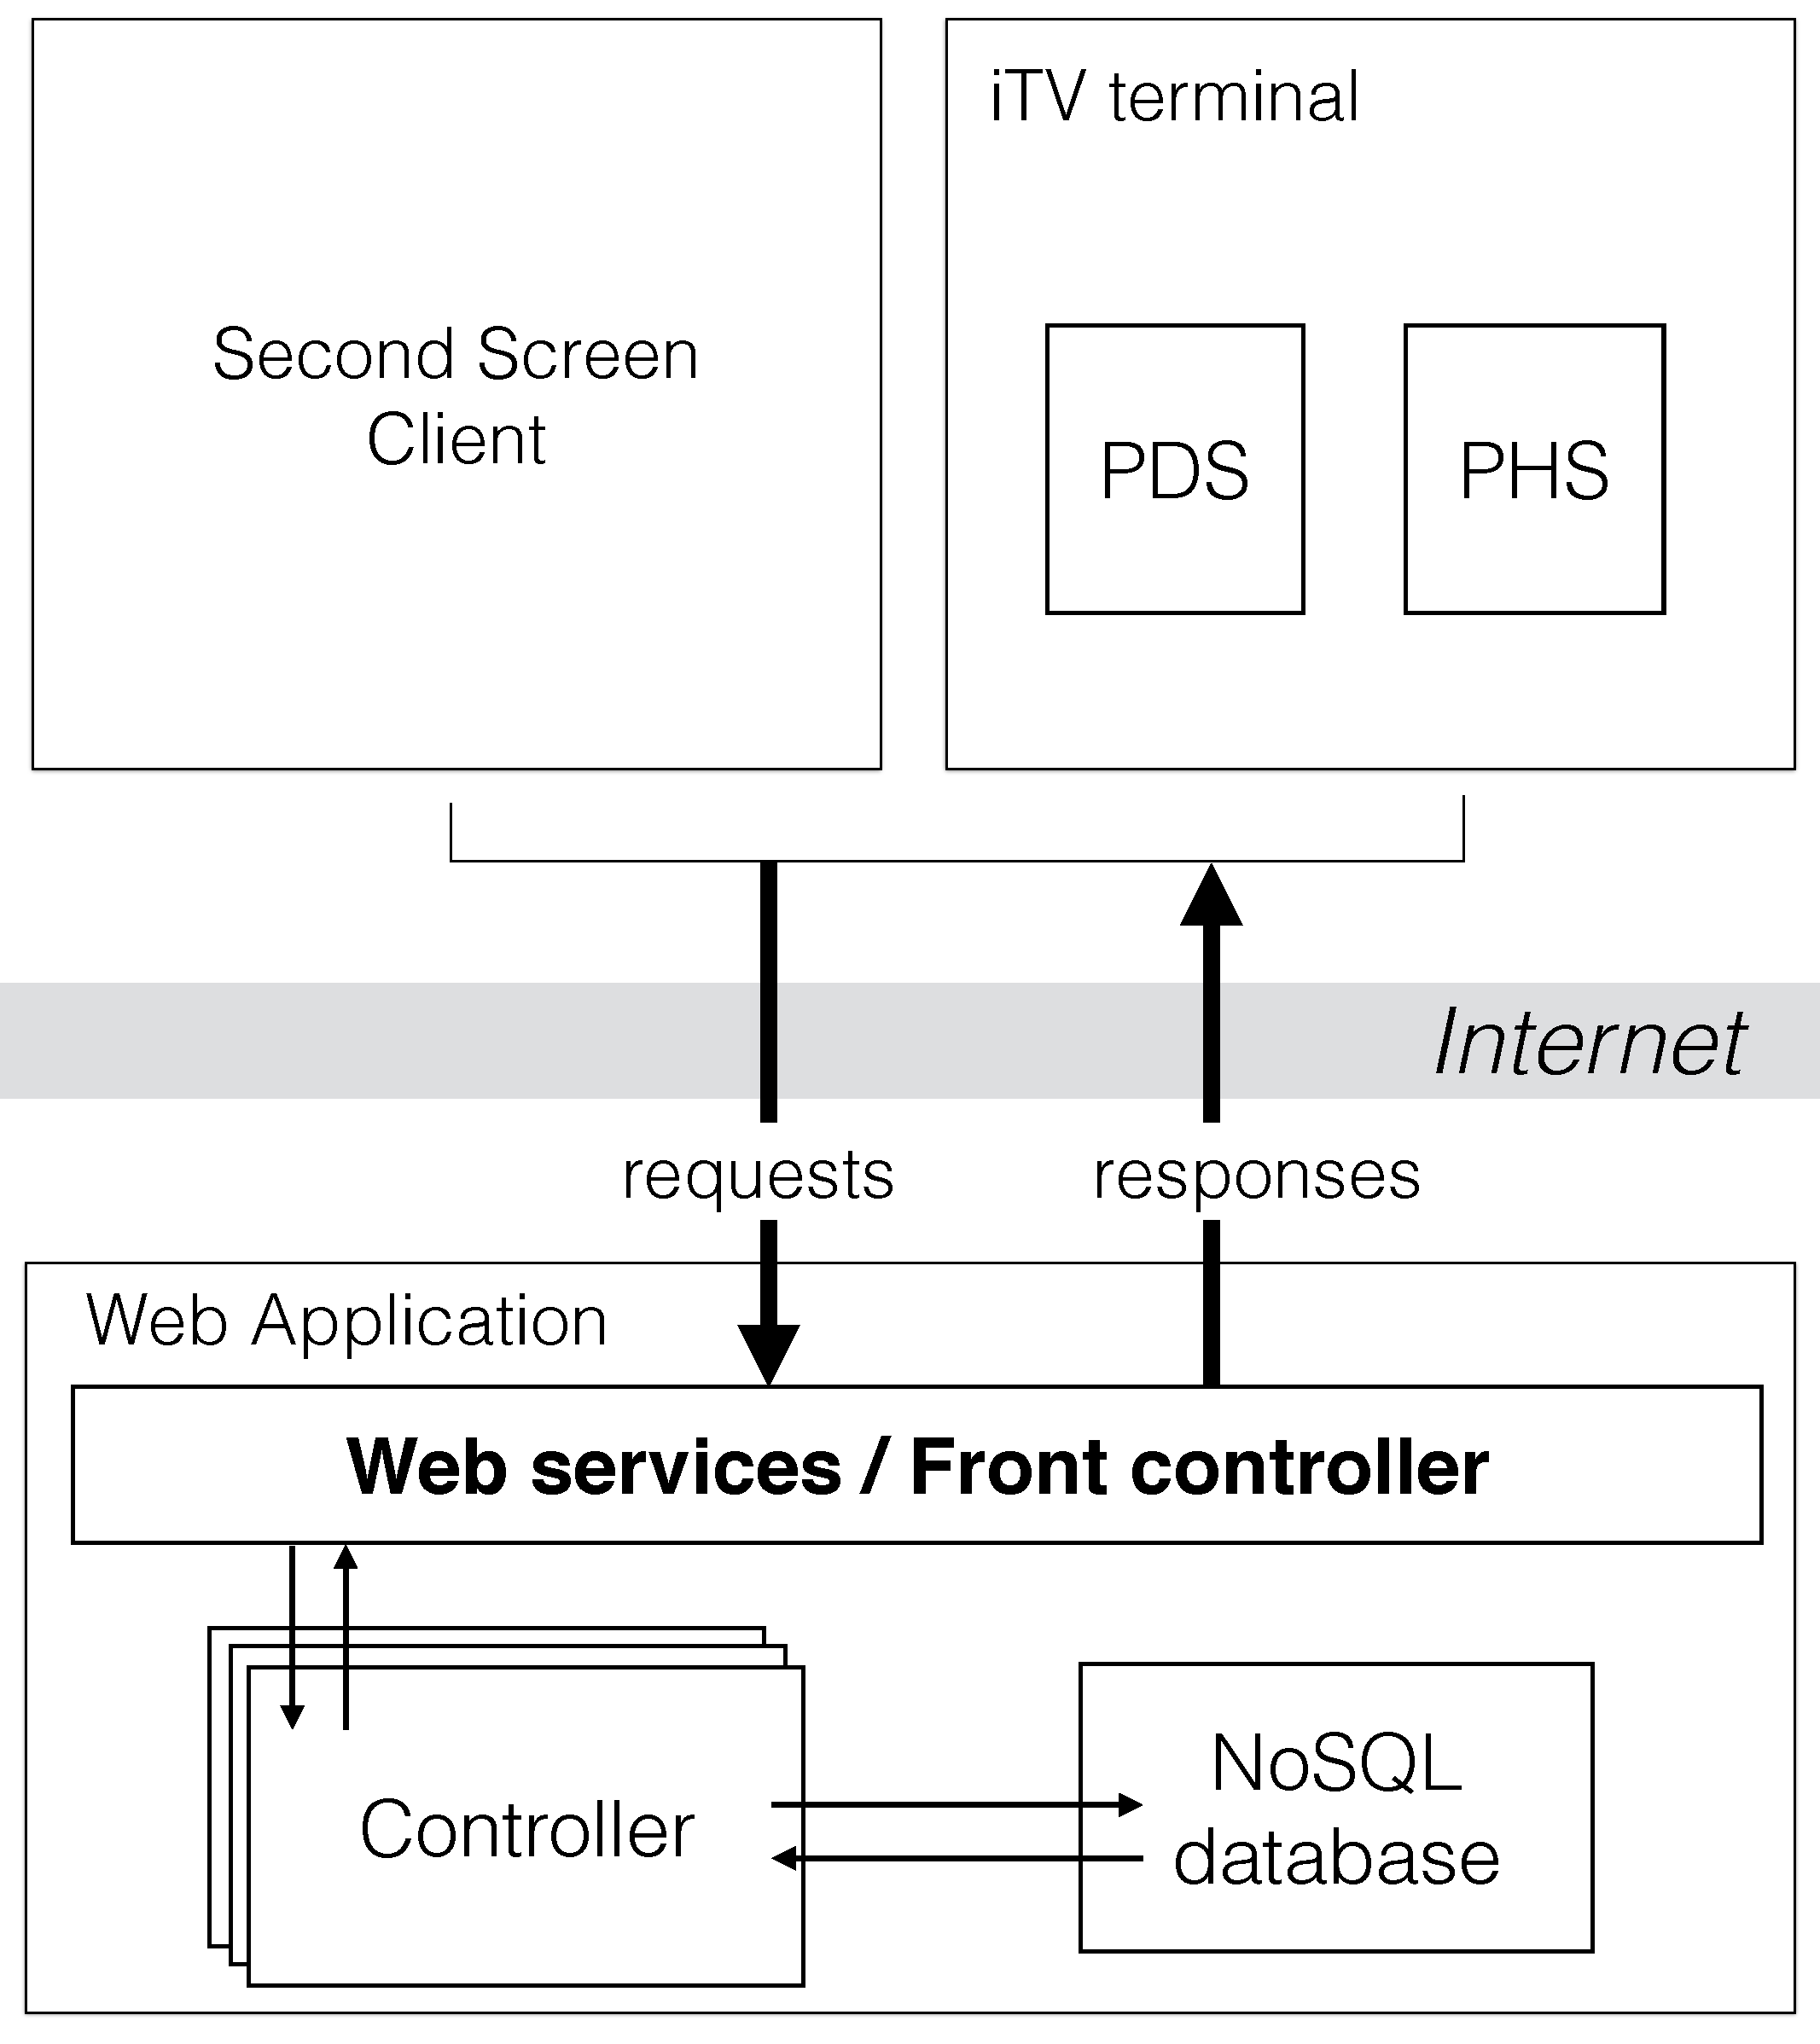
\includegraphics[width=3.5in]{img/architecture-overview.pdf}
	\caption{Architecture to capture audience interactions. The viewers' interactions and the contextual information are captured and stored in the CP infrastructure.}
	\label{fig_architecture}
\end{figure}

An overview of the architecture described in this paper is presented in \figurename~\ref{fig_architecture}. This architecture consists of tree subsystems that interact with each other: (1) second screen devices, which are personal devices; an (2) iTV terminal; and (3) the CP infrastructure. The CP infrastructure includes an application hosting infrastructure, which comprises the computing resources (e.g., application server, database services and storage services) that are necessary to host web applications. The dashed arrows represent the data flowing from the viewer to the CP infrastructure, while dotted arrows denote the flow from CP infrastructure to the viewers. The continuous arrows represent the data flow inside the CP infrastructure.

A web application is hosted in the application hosting infrastructure. This application contains web services that are designed for interoperability between the second screen devices, the iTV terminal and the CP infrastructure. A authentication mechanism must be provided so that the viewers can connect their second screen devices and interactive TV terminals (e.g., set-top boxes or smart TVs) with an user account. Once the authentication is completed, the second screen device can be used to interact with the iTV terminal.

A presence service detects physically nearby second screen devices that have the services necessary to establish a communication with an iTV terminal. This feature is particularly appropriate for the TV environment, once second screen devices are usually connected with an iTV terminal via WiFi. The devices are synchronized in order to update the contextual data about the viewer profile, amount of people using a second screen devices in the room and content being watched. This contextual data can be used to learn how a viewer behaves towards other viewers. For example, a viewer behaves in a particular way while watching TV alone and the same viewer behaves in a different way while watching in group.

The second screen devices and iTV terminals have client applications that consume the web services in order to present the content to the viewers. These client applications also use the web services as an interface to send interaction data to the CP. 

% descrever a possibilidade de autenticação em outra parte do texto: A possible way to do so is to generate a registration code for each equipment 

% commentar sobre a sincronização de contexto entre iTV terminals e second screen devices.


\section{Architecture to Capture Viewers' Interactions}
\label{sec_architecture}

Viewers can use their second screen device to interact with TV by evaluating, commenting, sharing, or even recommending TV content to other viewers. The data related to those actions are naturally provided by the viewers, as part of the interaction, when using interactive applications (developed by the CP) installed in their second screen devices. The interactions and the contextual data are represented by the audience data, which is sent to CP infrastructure through Internet. Then, a Data Writer service stores the audience data related to each particular viewer and the iTV device.

The Data Writer service in the application hosting infrastructure consists basically of web services that provide interoperability among second screen devices, iTV devices and the CP infrastructure. The main advantage of this approach is the independence of operating system and programming languages used in the personal devices.
 
Once the audience data is stored, the CP can use this data to derive valuable information about users' tastes. This information can be used to provide personalized content to viewers based on the current context. Thus, the personalized content can be delivered via Internet to the second screen device or even to the TV, depending on the context.

\subsection{Application Hosting Infrastructure}

The application hosting infrastructure (AHI) consists of a server environment that provides the necessary computing resources to run a web application and make it available to client applications. This infrastructure can be owned by the CP or it can be hired from a third party service provider. As a matter of fact, the web applications hosted in the AHI are responsible for providing the interactive content that can be accessed by the second screen clients. In addition, the web applications offer features to store and to process interaction data obtained from the viewers.

The TV domain has the potential of facing very different audience ratings. As a result, the amount of viewers using a particular iTV service can drastically change during the day. So, an important requirement for shared iTV services is to dynamically scale up and down the computing resources according to workload demands. Researchers have proposed novel ideas based on cloud-computing environments to tackle this requirement~\cite{Lee2010,Lai2011}. Since the architecture presented in this paper is intended to support a potentially large amount of viewers, the use of a cloud-computing infrastructure is considered in order to handle the requests from client applications.

\subsection{Web Application}
\label{ssub_web_application}

The web applications include the business logic, models and controllers that are necessary for the proper functioning of the second screen client application. The content that is presented in the client can be requested through HTTP requests to web services designed for this purpose. In addition, the data captured by second screen clients in the iTV environment can also be sent to the CP by using HTTP requests. 

The HTTP requests handling is carried out by using the front controller architectural design pattern~\cite{Buschmann2007}. It is employed to centralize requests processing in a single component, which facilitates the design and implementation of services for different second screen clients. As a result, client applications can access the same service even when they are developed for different operating systems in different programming languages.

\subsection{iTV Environment}

The iTV environment consists of an iTV terminal, which can be an set-top box or some iTV terminal with some sort of communication technology e.g., WiFi or Bluetooth. This environment has some services to facilitate the communication with second screen devices. The first one is the Presence Detector Service (PDS), which is in charge of discovering nearby second screen devices. The PDS is connected with another service known as Profile Handler Service (PHS), which aims to perform profile management at each moment when new second screen devices are found in the iTV environment.

% describe a device to device communication

\subsection{Second Screen Devices}

The second screen devices are clients that communicate with the web application in order to provide interactive capabilities with the content being watched in the TV terminal. The communication between second screen clients and the web application is made through HTTP requests to the web services. Basically, there are two types of communication between clients and the web application: retrieval the content from the web server and transmission of the captured interactions to the web server. Since these types communication occurs between client and a web server, Internet connection is required to accomplish the requests.

The retrieval of content from the web server happens when the client application performs a specially designed HTTP request aiming to obtain the content from a specified resource. The content obtained from this request is then shown by the client application on the second screen device.

The interactions captured from the viewers are transmitted to the web server by using the same principle of the retrieval of content. A HTTP request is sent to the web service. However, in this case, the request is designed to submit the data to a specified resource in order to be processed by the web application.

\subsection{iTV and Second Screen Devices Communication}

An important feature of the architecture described in this paper is the possibility of performing communication between iTV and second screen devices. This type of communication enable the discovery of devices that are physically nearby, i.e., devices on the same local network or not~\cite{Hellman2013}. Since people are typically carrying their phones with them, it is possible to manage who is present in the environment at a given moment.

The mobile devices industry provided several means to enable communication among devices (e.g., mobile devices and iTV terminals), which usually include network service discovery and peer-to-peer (P2P) connections. A useful way to find out nearby devices that are able to communicate is by using network service discovery. It consists of an application that can broadcast its name and connection information on the local network and identifies other devices running a service with which it can communicate.

An interesting P2P communication technology that is being adopted by many mobile devices manufactures is the Wi-Fi Direct~\cite{Hellman2013}. This technology enables Wi-Fi devices to connect directly without requiring an intermediate dedicated access point. This type of communication is based on Wi-Fi and is very similar to Bluetooth, except that it uses a higher speed and a range beyond the Bluetooth capabilities.

% Colocar um parágrafo falando da importância de saber quem está por perto.

\section{Implementation of the Second Screen Architecture}
\label{sec_implementation}

%The architecture described in this paper combines several concepts and technologies, e.g. second screen, interactive television, mobile applications, device to device communication and web technologies. 
An implementation of the architecture described in this paper was developed using the Java programming language in both sides of the architecture. However, the proposed approach does not require uniquely the Java programming language and the its use does not subtract the generality of the architecture. Indeed, the architecture can be implemented in other languages provided that they are compatible with the development platforms and with the concepts described in this paper.

\subsection{Web Services API Design and Implementation}

The second screen devices and the iTV terminals need to communicate with the web application in order to send viewer's interactions and retrieve content from the server. As defined in the Section~\ref{ssub_web_application}, this communication occurs by means of HTTP requests to the web services of the web application. Thus, an API containing the Uniform Resource Identifiers (URIs) and the HTTP methods available for each URI is needed.

\begin{table}
	\caption{Strategies to perform HTTP requests by combining URIs and HTTP methods.}
	\label{table_web_serv_design}
	\centering
	\begin{tabular}{|m{1.5cm}|>{\centering}m{1cm}|m{5cm}|}
	\hline
	\textbf{URI}&\textbf{HTTP method}&\textbf{Description of the HTTP request}\tabularnewline
	\hline
	/resources & GET & Retrieves a collection of resources of the same type that is specified in the URI. \tabularnewline
	\hline
	/resources/\{id\} & GET & Retrieves a single resource identified by a given \emph{\{id\}}.\tabularnewline
	\hline
	/resources & POST & Creates a new resource of the same type that is specified in the URI.\tabularnewline
	\hline
	/resources/\{id\} & PUT & Updates a resource identified by a given \emph{\{id\}}.\tabularnewline
	\hline
	/resources/\{id\} & DELETE & Deletes a resource identified by a given \emph{\{id\}}.
	\tabularnewline
	\hline
	\end{tabular}
\end{table}

Table~\ref{table_web_serv_design} describes how the web services API are designed by combining URIs and HTTP methods. The URI specifies the resource of interest and the HTTP method indicates the desired action to be performed on the resource. Since each HTTP method is intended for a different purpose, it is necessary to identify what actions apply to each resource.

A open source web framework~\cite{Wheeler2013} was used to develop the server side of the architecture, i.e., the web services. This framework facilitates the development of the front controller pattern in web-based application. Thus, all the requests are tunneled through a single entry point, which is an efficient mechanism to implement an API to access the web services. This mechanism not only routes and dispatches the requests to appropriate handlers, but also exposes a flexible and scalable API structure, which can be consumed by second screen devices using different programming languages.

\subsection{Web Service Consumption}

Since there is a well-defined web services API to access resources in the web application, it is possible to send HTTP requests from second screen devices and iTV terminals. A base URI which contains the domain of the web application (e.g., \emph{http://example.com}) is used as part of the API. Thus, the implementation of the HTTP requests in the client devices must use the entire URI, including the resource of interest.

The effect of the HTTP request depends on the type of HTTP method that is used, which typically can be GET, POST, PUT, or DELETE. Requests using GET must only retrieve data from the server. Depending on the URI, a request using GET should retrieve either a single element or a collection of elements of the specified resource. Responses bodies for requests using GET methods typically are in JSON format. However, it is also possible to provide other Internet media types, e.g., XML or Atom. Requests using POST demand that the server accept a new resource identified by the URI. Requests using PUT modify a resource identified by the URI. The requests using the DELETE method are intended to delete a resource specified by the URI.

The proper combination of URIs and HTTP methods is used to manipulate resources in HTTP requests. It is possible to implement CRUD (create, read, update and delete) operations that are intended for communication between the second screen devices and the web application. As a result, the client devices can consume the web services and perform the desired actions on the resources.As an example, a request can be used to send viewers' interactions to the web server, or to retrieve content that is personalized according past interactions of the viewer.

\section{Experiment: Evaluation of TV Programs using Second Screen}
\label{sec_experiment}

% Enfatizar a interação de avaliar um programa

To motivate the need for using this architecture in second screen-based iTV environments, a scenario that enables the viewer to evaluate TV programs was developed. This scenario uses mobile devices (second screen devices) to present content related to what is being watched on TV and capture viewers' interactions. To develop this scenario it was used a commercial cloud-computing environment intended for emulating the CP infrastructure and a mobile device with a commercial operating system.

The content that is presented in the mobile device is retrieved from a web server through Internet and is shown in an application, which was specially designed for second screen purposes. In this application, every time a viewer evaluates a TV program, the data obtained from this interaction is captured and sent to the web application through a HTTP request. This request carries data such as \emph{viewerId} (id of the viewer), \emph{programId} (id of the TV program), and \emph{rating} (a value from 1 to 5).

It is important to note that every type of interaction can be captured, e.g., viewers' navigation between TV programs, amount of time spent viewing information about a TV program on the second screen, time stamp of the interaction, and etc. However, it is necessary to attach triggers to the application so that every time an interaction occurs, the data obtained from this specific interaction is sent to the web application in a HTTP request.

\subsection{Implementation of the Web Application}

The web services API consists in handling three types of resources: viewers, TV programs and programs evaluations. The following URIs and HTTP methods describe some of the HTTP requests for viewers resources that were developed in this experiment:

\begin{itemize}
	\item \emph{/viewers} - POST: creates a new viewer, as identified by the resource that is present in the URI. The parameters that are carried in this type of request are \emph{viewerId}, \emph{username}, and \emph{password}.
	\item \emph{/viewers/\{viewerId\}} - GET: retrieves a specific viewer identified by \{viewerId\} in the URI. This request retrieves information about the viewer, which in this case are only \emph{viewerId} and \emph{username}, since is not safe to include a \emph{password} in the response body.
	\item \emph{/viewers/\{viewerId\}/evaluations} - GET: retrieves a collection of evaluations that were performed by a viewer identified by \{viewerId\}. Each evaluation contains a \emph{programId}, \emph{viewerId}, and a \emph{rating}.
\end{itemize}

HTTP requests for TV programs are identified as follows:

\begin{itemize}
	\item \emph{/programs} - POST: creates a new TV program, so that it is available to be presented in the second screen clients. In this experiment, an on-line videos platform was used provide videos to second screen clients. 
	\item \emph{/programs} - GET: retrieves a collection of TV programs that are available on the CP. A TV program representation contains a \emph{programId}, a \emph{videoCode} (id of the video on the videos platform), and \emph{title} (a title for the video representing the program).
	\item \emph{/program/\{programId\}} - GET: retrieves a single program identified by \emph{\{programId\}}.
\end{itemize}

Resources related to the evaluations performed by viewers are handled by the following HTTP requests:

\begin{itemize}
	\item \emph{/evaluations} - POST: creates a new evaluation. This HTTP request requires three attributes: \emph{viewerId}, \emph{programId}, and \emph{rating}.
	\item \emph{/evaluations/viewers/\{viewerId\}/programs/\{programId\}} - GET: retrieves an evaluation of a viewer identified by \emph{\{viewerId\}} on a given TV program identified by \emph{\{programId\}}.
\end{itemize}

Some of the HTTP requests were created only to add content to the web application, so that the client devices could access this content. The client devices typically use GET method in HTTP requests to retrieve content from the web application. In this experiment, the responses to the HTTP requests were provided in the JSON format. \figurename{~\ref{fig_response_json}} presents a JSON representation of a resource obtained with an HTTP request to \emph{/evaluations/viewers/\{viewerId\}/programs/\{programId\}} using a GET method. The implementation of this request searches for a resource of the type evaluation that has a \emph{\{viewerId\}} equals to 5629499534213120, and a \emph{\{programId\}} equals to 5649391675244544.

\begin{figure}
\begin{verbatim}
{
    id: 5722646637445120,
    viewer: {
        id: 5629499534213120,
        username: "user1"
    },
    program: {
        id: 5649391675244544,
        videoCode: "ZuQ4obQAN8",
        title: "A Program Title"
    },
    rating: 4
}
\end{verbatim}
\caption{Response to an HTTP request using GET method in JSON format. The code shown in this figure is a JSON representation of a resource of the type evaluation.}
\label{fig_response_json}
\end{figure}

\subsection{Implementation of the Second Screen Application}

Lorem ipsum dolor sit amet, consectetur adipisicing elit, sed do eiusmod
tempor incididunt ut labore et dolore magna aliqua. Ut enim ad minim veniam,
quis nostrud exercitation ullamco laboris nisi ut aliquip ex ea commodo
consequat. Duis aute irure dolor in reprehenderit in voluptate velit esse
cillum dolore eu fugiat nulla pariatur. Excepteur sint occaecat cupidatat non
proident, sunt in culpa qui officia deserunt mollit anim id est laborum.

\section{Conclusions}
\label{sec_conclusions}

The use of personal devices as second screens arises as a new trend in TV environments. This paper presents an architecture to accurately capture audience data by using second screen devices and iTV devices. This architecture take advantage of the ubiquity and interactive capabilities of second screen devices to identify viewers and provide feedback for CPs through viewers' interactions and contextual information. The captured data relates to a single viewer in a given context. By using proper machine learning algorithms, this data can provide valuable information about viewers. Knowing this information can be very useful for CPs to improve their services aiming to increase the audience and to enrich user experience. As an example, CPs can deliver personalized content for a single person as well as for groups of people by using content recommendation algorithms.

An implementation of the architecture that is described in this paper is under development in a commercial cloud computing platform, which plays the role of the application hosting infrastructure. A web application that consists of a content rating system was developed to store  viewers' evaluations toward audio visual content, and a second screen client is under development. Some RESTful web services were developed to provide interoperability among the second screen devices and the web application. Thus, the interactions that are captured during the use of the second screen application are sent to the CP by means of HTTP requests to RESTful web services. Although the second screen application is not fully finished yet, some specific features have been tested to capture viewers' interactions as they occur.

The architecture described in this paper is also technically feasible to implement in Digital TV (DTV) systems and can be particularly interesting for CPs in DTV standards, e.g., the Brazilian (ISDB-TB) and the Japanese(ISDB-T). These standards support the use of mobile devices as part of the system. Since the mobile devices support the implementation of the DTV middleware, a cooperative exhibition of the DTV application can be managed with the iTV device, thus enabling the capture of viewers' interactions and contextual data.

% Nowadays, viewers rarely just sit passively and watch TV. In many situations, they use their personal devices as a secondary screen to perform activities related to TV watching, which end up enriching and immersing the user into the TV experience. 


\bibliographystyle{IEEEtran}
\bibliography{biblio}

\end{document}